\section{Information Fusion}
\label{sec:2_4_fusion}
In any estimation process, having information from different sources is always positive.
As a general rule, merging several estimates does not always improve the accuracy of the estimate. 
However, the precision of the estimate will always be better than the precisions of the individual estimates.
This may be important for applications that may admit some error in estimation but require certain levels of integrity or confidence in the estimates.
The merging of information can be done from various points of view:
\newpage
\begin{description}
	\item \textbf{Integration of several systems or technologies}
	
	When integrating several localization systems, a first strategy may be to use several systems with similar characteristics, in a redundant manner, such as a foot-mounted INS on each foot \cite{prateek_data_2013} or to combine a foot-mounted INS with a PDR carried in the pocket of the pants \cite{bousdar_ahmed_loose_2017}.
	In this way, the estimation of the position may be improved but the overall system will continue to have the same types of weaknesses.
	
	A fusion strategy that seems more interesting is to combine systems or technologies that have complementary characteristics.
	A simple example in relation to the coverage requirement could be the use of GNSS for outdoors scenarios and WLAN access points for indoors.
	
	However, the most powerful strategy is to merge localization systems based on different methods, i.e. position fixing and DR.
	Remembering the main strengths and weaknesses of each type of method, it can be seen that they complement each other perfectly.
	DR based methods are scenario independent, have a good short-term accuracy but their errors accumulate unbounded over time.
	Meanwhile, position fixing based methods have bounded errors in the long-term but with a risk of temporary higher errors due to interferences or complicated scenarios. In addition, they depend on the infrastructure installed on the scenario.
	
	The most common example of this strategy is the fusion of GNSS and INS systems.
	Furthermore, this integration can be done at different levels, depending on whether only the solutions of each systems is fused (loose coupling) or whether the fusion occurs during the estimation process (tight coupling and deep integration). 
	Detailed descriptions can be found in references \cite{grewal_global_2001, titterton_strapdown_2004, groves_principles_2008}.		

	\item \textbf{Prior knowledge}
		
	Another source of information that can be merged to improve estimates is the available a priori knowledge about the use case, which can be of different types:	
	\begin{itemize}
		\item Information about movement restrictions:
				As previously discussed in Section~\ref{sec:2_3_1_3_DR_INS_ZUPT}, it is possible to use the knowledge about the characteristics of the motion to correct the estimation errors, being two of the best known techniques ZUPT and ZARU, which both make use of the moments when the feet are still on the ground.
				
				Another technique, known as \emph{Heuristic Drift Reduction} (HDR) \cite{borenstein_heuristic_2009}, is to assume that people usually walk in a straight line, especially inside buildings, which allows to reduce the drift in the heading.				
		\item Information about the navigation scenario:
				Having information about the spatial distribution of the characteristics of a certain area is not sufficient to localize an object, but it can be useful to improve the estimation obtained by other means.
				The clearest example is having the map of a building. In addition to assisting in visualization, it can be used to apply corrections to the position estimation, both by using the complete building structure, such as in \cite{woodman_pedestrian_2008, xiao_lightweight_2014, bataineh_conditional_2016}, the detection of landmarks of known position such as stairs, elevators, ramps \cite{jimenez_pdr_2011}, or by the detection of activities performed by the user that may be related to a certain position, such as opening a door.
				
				Similar to the HDR technique mentioned in the previous point, in addition to assuming straight sections in a building, it is also possible to use the ``dominant'' directions of the corridors of a building to correct the heading drift \cite{borenstein_heuristic_2010, abdulrahim_aiding_2010, jimenez_improved_2011, jimenez_improved_2012}. 
				%This technique, and its derivatives, are usually known as \emph{Heuristic Drift Elimination} (HDE) \cite{borenstein_heuristic_2010, abdulrahim_aiding_2010, jimenez_improved_2011, jimenez_improved_2012}.				
				Such techniques will be discussed in Chapter~\ref{cha:9_ihde}.
				
				A more advanced technique is to simultaneously generate a landmark map while locating the object on that map. 
				This technique is known as \emph{Simultaneous Localization And Mapping} (SLAM) and has been widely used in robotics \cite{durrant-whyte_simultaneous_2006}.				
	\end{itemize}	
	\item \textbf{Dynamic estimation}	
	
	The estimation methods for position fixing based localization systems seen in Section~\ref{sec:2_2_2_techniques} assumed that the set of measurements received had been generated when the object was in the same position. This is equivalent to the object being static.
	When the object is in motion, fewer measurements will generally be available at each position, so the estimate will tend to be worse.
	However, it is possible to extend the estimation process by trying to use all the measurements received up to that moment. 	
	For this, it is necessary to have information about the dynamics of the moving object, so that it allows ``linking'' the previous measurements and position estimates with the current one, thus improving the estimation of the moving object.
	
	The mathematical tool that is usually used for this type of information fusion is the Bayesian filtering. 
	Given their importance and frequency of use in the field of localization, the following section introduces the main concepts and techniques.	
\end{description}		
%%%%%%%%%%%%%%%%%%%%%%%%%%%%%%%%%%%%%%%%%%%%%%%%%%%
\subsection{Bayesian Filters}
\label{sec:2_4_1_fusion_bayesian}
The basic idea is to propose that the probability density function of the estimation of the current position of the object, that is, its uncertainty, can be defined as the probability a posteriori conditioned to all the measurements received up to that moment $t$:
\begin{equation}
\label{eqn_bayes_cond}
	p(\boldsymbol{x}_t)=p(\boldsymbol{x}_t|\boldsymbol{z}_1, \boldsymbol{z}_2,...,\boldsymbol{z}_t)
\end{equation}
In general, the complexity of computing such posterior densities grows exponentially over time, since more measurements will be available.
To reduce that complexity, Bayesian filters assume that the dynamic of the system is a Markov process.
Translated to the localization scope, this means that it is possible to make predictions of future positions based solely on the current position, as it contains all the information about its status. In other words, the positions and measurements of the past do not provide additional information.

Under Markov's process condition, it is possible to convert the equation~\ref{eqn_bayes_cond} into an iterative process, based on two phases.
First, the filter predicts the next position from the current estimate of $\boldsymbol{x}_{t-1}$
\begin{equation}
\label{eqn_bayes_pred}
	p^{-}(\boldsymbol{x}_t)=\int p(\boldsymbol{x}_t|\boldsymbol{x}_{t-1})p(\boldsymbol{x}_{t-1})d\boldsymbol{x}
\end{equation}
where $p(\boldsymbol{x}_t|\boldsymbol{x}_{t-1})$ represents the object's dynamic model, that is, how its position varies over time.

The correction phase then merges the newly obtained prediction with the measurements obtained in the period between $t-1$ and $t$. 
By applying the Bayes rule, the posterior probability is obtained as:
\begin{equation}
\label{eqn_bayes_corr}
	p(\boldsymbol{x}_t)=p(\boldsymbol{x}_t|z_t)=\frac{p(\boldsymbol{z}_t|\boldsymbol{x}_{t})p^{-}(\boldsymbol{x}_t)}{p(\boldsymbol{z}_t)}
\end{equation}
where $p(\boldsymbol{z}_t|\boldsymbol{x}_{t})$ is the observation model and the measurement probability $p(\boldsymbol{z}_t)$ normalizes the product for ensuring that the posterior over the entire state space sums up to one:
\begin{equation}
\label{eqn_bayes_norm}
	p(\boldsymbol{z}_t)=\int p(\boldsymbol{z}_t|\boldsymbol{x}^{-}_{t})p(\boldsymbol{x}^{-}_{t})d\boldsymbol{x^{-}}
\end{equation}

In this probabilistic model, $\boldsymbol{x}_{t}$ represents a state vector, so it may contain additional variables to the position such as velocity, orientation or the inertial sensor biases.
In addition, since its formulation is done considering generic probability density functions, it facilitates the fusion of measurements from different types of sensors in a probabilistic way.

The calculation of the different integrals can be difficult to perform in real time. For this reason, there are different simplified implementations of this Bayesian formulation for certain specific cases:
\begin{description}
	\item \textbf{Kalman Filter}

	The simplest case is the \emph{Kalman Filter} (KF), which is based on a state-space representation of the dynamic system in discrete time, and it can be shown that it is the optimal estimator when the error distributions are Gaussian and the observation and dynamic models are linear function of the state vector.
	Although the original derivation of the KF used the orthogonality principle and iterative updates to find the best linear unbiased estimator, it can also be derived using a Bayesian approach, where ``best'' is interpreted in the maximum a posteriori sense, since for Gaussian errors is the same estimate.
	
	So, since a Gaussian distribution is completely described by the mean and the covariance, the prediction stage has the following form:
	\begin{equation} % El & para que se alineen a nivel del =
	\label{eqn_KF_pred}
		\begin{aligned}
			\boldsymbol{x}^{-}(k)&=\boldsymbol{F} \cdot \boldsymbol{x}(k-1)\\
			\boldsymbol{P}^{-}(k)&=\boldsymbol{F} \cdot \boldsymbol{P}(k-1) \cdot \boldsymbol{F}^T+\boldsymbol{Q}
		\end{aligned}
	\end{equation}		
	where $\boldsymbol{x}^{-}(k)$ and $\boldsymbol{P}^{-}(k)$ are the predicted mean and covariance matrix, respectively, $\boldsymbol{F}$ is the state transition matrix and $\boldsymbol{Q}$ is the covariance matrix of the process noise.
	
	The correction stage will use the observed $\boldsymbol{z}$ measurements with its $\boldsymbol{R}$ covariance matrix for modeling the measurement noise:
	\begin{equation} % El & para que se alineen a nivel del =
	\label{eqn_KF_corr}
		\begin{aligned}
			\boldsymbol{x}(k)&=\boldsymbol{x}^{-}(k)+\boldsymbol{K}\cdot (\boldsymbol{z}-\boldsymbol{H}\cdot \boldsymbol{x}^{-}(k))\\
			\boldsymbol{P}(k)&=(\boldsymbol{I}-\boldsymbol{K}\cdot\boldsymbol{H})\cdot \boldsymbol{P}^{-}(k)
		\end{aligned}
	\end{equation}		
	where $\boldsymbol{H}$ is the observation matrix and $\boldsymbol{K}$ is the Kalman constant:
	\begin{equation}
	\label{eqn_KF_K}
		\boldsymbol{K}=\boldsymbol{H}^T \cdot \boldsymbol{P}^{-}(k) \cdot (\boldsymbol{H}^T  \cdot \boldsymbol{P}^{-}(k) \cdot \boldsymbol{H}+\boldsymbol{R})^{-1}
	\end{equation}		
	
	\item \textbf{Extended and Unscented Kalman Filter}	
	
	When some of the KF assumptions, i.e. linearity and normality, are not fully met, modified versions of the KF are usually used which, although sub-optimal, achieve good accuracies.
	
	The first of these is the \emph{Extended Kalman Filter} (EKF), which is based on the linearization of the dynamic and observation models, achieving a similar formulation in which the main difference is the use of the Jacobian matrices of those models, in which only the first terms of their Taylor series are taken.
	
	The other variant is known as \emph{Unscented Kalman Filter} (UKF), which is based on propagating over time a sampling of the mean and covariance of the state vector, which are known as ``sigma'' points. Through this process, states are propagated to the third order terms of their Taylor series, allowing for better estimates and faster convergence.	
	\item \textbf{Particle Filter}
		
	When linearity or normality conditions are not significantly met, non-pa\-ram\-e\-tric filters, such as \emph{Particle Filters} (PF), are often used.
	These filters do not assume any dynamic and observational models and are based on propagating a sampling of the probability distribution of the state vector over time.
	The main objective is to propagate only the most likely points of the sample, eliminating the most unlikely ones in order to reduce the complexity of the calculation.
	This technique is very flexible in terms of the type of measurements that can be used in the observation model, which is why it is usually the technique chosen to include highly non-linear information, such as map-matching information.	
	
\end{description}
There are good references explaining these techniques in detail (KF/EKF \cite{kalman_new_1960,bishop_introduction_2001}; UKF \cite{julier_new_1997};PF\cite{arnaud_tutorial_2008}) and their use in localization \cite{fox_bayesian_2003, seco_survey_2009}.
%%%%%%%%%%%%%%%%%%%%%%%%%%%%%%%%%%%%%%%%%%%%%%%%%%%
\section{Attitude and Heading Reference Systems}
\label{sec:2_5_AHRS}
An \emph{Attitude and Heading Reference System} (AHRS) is like a sub-module of an INS: it only tracks the orientation of the object by integrating the angular rates provided by a set of gyroscopes.
Therefore, in the same way, the orientation error also accumulates over time and information from other type of sensors is usually fused to reduce or reset the error.
Early AHRS designs were based on deterministic fusion strategies and they commonly used accelerometers for reseting the object's tilt, provided that it is static, and magnetometers for the heading \cite{mahony_nonlinear_2008, madgwick_efficient_2010}.
%However, since the use of the values provided by the magnetometers as true heading is mainly restricted to outdoors, last AHRS proposals tend to choose probabilist fusion strategies and limit the use the magnetometers for estimating the gyroscopes bias whenever a constant magnetic field is detected \cite{munoz_diaz_use_2017}.
However, since the use of magnetometers to calculate the actual heading can only be reliably performed outdoors, more recent AHRS tend to choose probabilist fusion strategies and only use such sensors to estimate the bias of the gyroscopes whenever a constant magnetic field is detected \cite{munoz_diaz_use_2017}.

As mentioned in a previous section, the orientation of an object with respect to a reference frame can be represented in several ways: rotation matrix, Euler angles and quaternions.
% Las representaciones son equivalentes pero cada una tiene sus pros y sus contras: 
% \begin{itemize}
	% \item Las matrices de rotación, también llamadas direction cosine matrices, son una matriz de 3x3 cuyas columnas representan la proyección del body reference sobre el global reference. Su principal ventaja es que la matemática de matrices es bien conocida y, además, facilita realizar transformaciones como proyecciones, escalados o traslaciones. Por contra, sus principales desventajas es que no permite visualizar intuitivamente la rotación y que es una representación redundante, ya que utiliza nueve valores para representar tres grados de libertad.
	% \item Leonard Euler demonstrated that the orientation of a rigid body with respect to a fixed reference system can be defined as a sequence of three elementary rotations. Su principal ventaja es que sólo es necesario almacenar esos tres valores y que, conociendo la secuencia de rotación, es sencillo visualizar la rotación total. Por contra, sus mayores problemas son que para operar matemáticamente se deben transformar a matrices de rotación y que algunas secuencias de rotaciones pueden generar una singularidad en la que se pierde un grado de libetad. Esta situación es llamada gimbal lock.
	% \item Los quaternions son una extensión de los números complejos definidos por cuatro parámetros y que permiten representar una orientación como una única rotación alrededor de un eje concreto. Sus ventajas es que son más eficientes que las matrices de rotación y no sufren el problema de gimbal lock de los Euler angles. Sin embargo, tampoco es intuitivo visualizar la rotación a partir de ellos.
% \end{itemize}
These three representations are equivalent as it is possible to convert each one into the others. However, each one has its pros and cons \cite{shuster_survey_1993}: 
\begin{itemize}
	\item The rotation matrices, also called direction cosine matrices, are a three-by-three matrix whose columns represent the projection of the body reference vectors on the global reference. Its main advantages are that matrix mathematics is well known and that it is easy to perform transformations such as projections, scaling or translations. 
	On the other hand, its main disadvantages are that it is not intuitive to visualize the orientation from the matrix expression. Additionally, it is a redundant representation, since it uses nine values to represent three degrees of freedom.
	\item Leonard Euler demonstrated that the orientation of a rigid body with respect to a fixed reference system can be defined as a sequence of three elementary rotations, the so-called Euler angles. 
	The main advantage of this representation is that it is very efficient since only three values are necessary and that, knowing the rotation sequence, it is easy to visualize the orientation. 
	On the other hand, the main problems are that to operate mathematically they must be transformed into rotation matrices and that some rotation sequences can generate a singularity in which a degree of freedom is lost. This situation is called gimbal lock.
	\item The quaternions are an extension of the complex numbers, defined by four parameters.
	They allow to represent an orientation as a single rotation around a particular axis. 
	Their advantages are their numerical efficiency with respect to the rotation matrices and that they do not suffer from Euler angles' gimbal lock problem. 
	However, it is also not intuitive to visualize the orientation from its values.
\end{itemize}
\begin{figure}[!t]
	\centering
	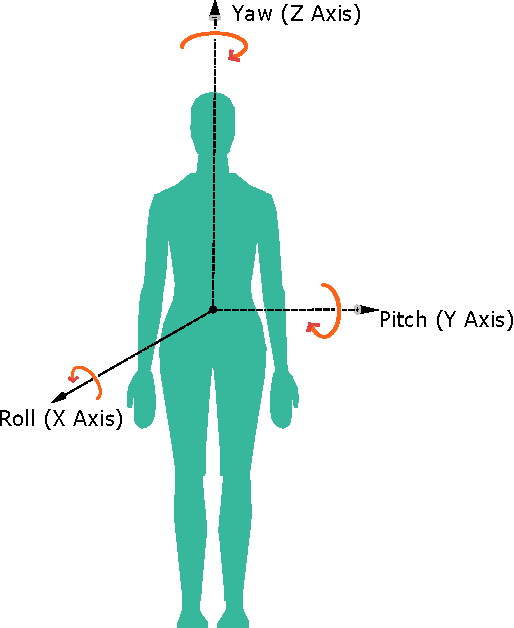
\includegraphics[scale=1]{Yaw_Axis_Corrected_human}
	\caption[Definition of roll, pitch and yaw angles]{Definition of roll, pitch and yaw angles: although there may be variations depending on the definition of the body and global reference systems, in general, the yaw is measured in relation to the vertical axis and indicates the direction that the body faces, the pitch is measured in relation to the lateral axis and indicates the body's elevation, and the roll is measured in relation to the anteroposterior axis.}
	\label{fig:Euler}
\end{figure}
For these reasons, during the mathematical formulation of INS strapdown mechanization, rotation matrices were used.
In contrast, AHRS systems usually use Euler angles when their estimation is to be shown to the user.
So, back to the Euler angles, there are 12 possible rotation sequences, defined with respect to the axes of the body's reference system. 
One of the most common one is the ``ZYX'' sequence, whose three angles are usually known as yaw, pitch and roll \cite{noauthor_ieee_2009}.
As can be seen in the Figure~\ref{fig:Euler}, yaw is the rotation angle around the vertical ``Z'' axis of the body. The term heading is sometimes used as a synonym but it is the angle to the north direction, while yaw is with respect to a reference frame which may not be north-facing.
Pitch, also called elevation, indicates the rotation around the lateral axis ``Y''.
And, finally, the roll angle, also called bank, is around the anteroposterior axis ``X''.
%A visual example of these three Euler angles can be seen in the Figure~\ref{fig:Euler}.
%For this sequence, and as can be seen in the Figure~\ref{fig:Euler}, these 3 angles are usually known as \cite{noauthor_ieee_2009}:
% \begin{itemize}
	% \item Yaw: rotation around the vertical ``Z'' axis. The term heading is sometimes used as a synonym but there is a small difference. Heading is the angle to the north direction. Yaw, on the other hand, is the angle to longitudinal axis of the reference system, which may not be north-facing.
	% \item Pitch: rotation around the lateral axis ``Y''. Also called elevation.
	% \item Roll: rotation around the lateral axis ``X''. Also called bank.	
% \end{itemize}
%\InsertFig{Yaw_Axis_Corrected.pdf}{fig:Euler}{Definition of roll, pitch and yaw angles}{Source: \cite{jrvz_english:_2010}}{0.75}{}
%\InsertFig{Yaw_Axis_Corrected_human.pdf}{fig:Euler}{Definition of roll, pitch and yaw angles}{}{1}{}

PDR systems usually have an AHRS to have a continuous estimation of the heading and, from it, to determine the heading of each step or stride.
In addition, there are also systems that use the Euler angles signals as a source of information for detecting the steps or estimating their length. This is because, depending on where the IMU is mounted, these angles can provide a lot of information about the position of some segments of the human body.